\documentclass[12pt, 
    twoside=false, 
    bibliography=totoc, 
    numbers=endperiod, 
    headings=normal, 
    toc=chapterentrydotfill
    ]{scrbook}
\usepackage[utf8]{inputenc}
\usepackage[ngerman]{babel}
\usepackage{blindtext}
\usepackage{csquotes}
\usepackage{booktabs}
\usepackage{setspace}
\usepackage{mathpazo}
\usepackage{graphicx}
\usepackage{etoolbox}
\usepackage[
  	pdfstartview=FitH,   
  	pdffitwindow=true,
  	colorlinks,
  	linkcolor=black,
  	anchorcolor=black,
  	citecolor=black,
  	urlcolor=black
  	]{hyperref}
\usepackage[labelfont=bf]{caption}
\usepackage{float}
\usepackage[
    backend=biber, 
    style=authoryear-ibid, 
    eprint=false,
    url=false,
    doi=false,
    isbn=false
    ]{biblatex}
\addbibresource{Bib.bib}

% Layoutanpassungen
\setkomafont{sectioning}{\normalcolor\bfseries}
\renewcommand*{\chapterheadstartvskip}{\vspace*{-\topskip}}
\KOMAoptions{headsepline = true}
\setlength{\textheight}{1.05\textheight}
\AtBeginEnvironment{quote}{\singlespacing\small}

\begin{document}

\begin{titlepage}
    \begin{minipage}[t]{0.6\textwidth}
    \flushleft 
    Universität Hamburg \\
    Fachbereich: Sozialwissenschaften \\
    Fachgebiet: Politikwissenschaft \\
    Seminar: Forschungsseminar Vergleichende und Regionalstudien \\ 
    Dozenten: Prof. Kai-Uwe Schnapp \\
    PD Dr. Falk Daviter \\
    Wintersemester 2018/19 \\
    \end{minipage}
    \hfill
    \begin{minipage}[t][1.7cm][b]{0.35\textwidth}
    
\includegraphics[width=\textwidth]{images/UHH-Logo_2010_Farbe_CMYK.pdf}
    \end{minipage}
    
    \vspace*{\fill}
    \begin{center}
	\vspace{1cm}\noindent {\textbf{Projektarbeit}} \vspace{0.2cm} \\
	\textbf{\Large Geschlechterunterschiede} \\
	\textbf{WIP} \\
	\vspace{0.2cm}
	30.03.2019
	\end{center}
    \vspace*{\fill}
	
	\begin{minipage}[t]{0.48\textwidth}
    \flushleft 
    Gina-Gabriela Görner \\
    Matrikelnummer: XXX \\
    XXX \vspace{0.1cm} \\ 
	XXX \vspace{0.1cm}  \\
	E-Mail: XXX \\ 
    \end{minipage}
    \begin{minipage}[t]{0.48\textwidth}
	\flushleft
	Josef Holnburger \\
	Matrikelnummer: XXX \\
	XXX \vspace{0.1cm} \\
	XXX \vspace{0.1cm} \\
	E-Mail: josef@holnburger.com \\
    \end{minipage}

\end{titlepage}

\frontmatter

\tableofcontents

\listoffigures
\addcontentsline{toc}{chapter}{\listfigurename}
\vspace*{24pt}
{\let\clearpage\relax \listoftables}	
\addcontentsline{toc}{chapter}{\listtablename}

\mainmatter

\setstretch{1.5}

\chapter{Einleitung}\label{Einleitung} 

Eine Vielzahl an Studien beschäftigt sich mit den Repräsentations- und Partizipationsunterschieden von Frauen und Männern in Parlamenten \parencite[416]{blaxill_2016}. Eine umfassende Untersuchung von Geschlechterunterschieden in Bezug auf Sprache, Thematik sowie Verhalten der Parlamentsmitglieder des Deutschen Bundestages ist allerdings bis zu diesem Zeitpunkt noch ausstehend. 

Anne Phillips gilt als eine der wichtigsten Vertreterinnen auf dem Gebiet der parlamentarischen Representativität von Frauen. In ihrem Werk "The Politics of Presence" analyisiert Phillips \parencite*{phillips_1998} unter anderem die Bereitschaft von Frauen, als Parlamentskandidatin ausgewählt zu werden, Ministerin zu werden und Wahlen zu gewinnen \parencite[vgl.][416f.]{blaxill_2016}. 
Da Frauen im täglichen Leben andere Erfahrungen sammeln als Männer -- insbesondere bezüglich der Kindererziehung, Bildung sowie der Auswahl an Berufen und der Spalting in bezahlte und unbezahlte Arbeit, Gewalterfahrungen sowie sexuellen Belästigungen -- plädierte Philips für die notwendige Repräsentation von Frauen im Parlament, um andere Frauen vertreten zu können und diese Situationen sichtbar zu machen \parencite[vgl.][52]{wangnerud_2009}.

\begin{quote}
    \enquote{There are particular needs, interests, and concerns that arise from women's experience, and these will be inadequately addressed in a politics that is dominated by men. Equal rights to a vote have not proved strong enough to deal with this problem; there must also be equality among those elected to once} \parencite[66]{phillips_1998}
\end{quote}

Die Theorie der \emph{politics of presence} \parencite{phillips_1998} diente Wängnerud \parencite*{wangnerud_2000} als Ausgangspunkt für ihre Forschung im Schwedischen Parlament (\enquote{Testing the Politics of Presence, Women's Representation in the Swedish Riksdag}, 2000). Wägnerud konzentriert sich hierbei auf die Repräsentation von Frauen und prüft die Hypothese, dass weibliche Politikerinnen die Interessen von Frauen stärker vertreten als männliche Politiker \parencite[84]{wangnerud_2000}. \enquote{[It is] difficult to repudiate the conclusion that women's interes are primarily represented by female politicians} \parencite[][84]{wangnerud_2000}.
Folglich tritt die Zahl der Frauen im Parlament zunehmen in den Vordergrund der wissenschaftlichen Auseinandersetzung und der Politik. 

Bei der Forschung zu Frauen im Parlament wird generell zwischen einer deskriptiven und einer substantiellen Repräsentation (in einigen Fällen außerdem die symoblische Form der Repräsenttation) unterschieden. Bei der substantiellen Repräsentation von Frauen handelt es sich um ein bisher weniger wissenschaftlich erforschtes Feld als die Analyse der deskriptiven Repräsentation \parencite[59]{wangnerud_2009}. Letzteres legt den Schwerpunkt auf die Analyse der Anzahl von Frauen in representativen Institutionen, ersteres untersucht hingegen die Auswirkung der Präsenz von Frauen in Parlamenten \parencites[14]{coffe_2013}[52]{wangnerud_2009}.
Die zentrale Fragen lauten hierbei:


\begin{quote}
  \enquote{[W]hether the widely professed aspiration to feminise democracy -- and in so doing to politically empower women -- is a matter largely of symbolism or substance […]}
  
  
  \enquote{[…] wheter the priority should simply be to increase the proportion of women MPs in Parliament […] or as Hanna Pitkin argued in 1967, to represent minds as well as bodies.}
  \parencite[413]{blaxill_2016}
\end{quote}

Bereits Piktin \parencite*{pitkin_1972} argumentierte in ihrem Hauptwerk "The Concept of Representation", dass der Interessenbegriff in der Repräsentationsdebatte omnipräsent ("ubiquitious") ist \parencite[69]{wangnerud_2000}. Für Pitkin sind es die Parliamentarierinnen, welche sich den Wünschen und Interessen, dem Wohlergehen sowie Themen der Frauen widmen und diese vertreten \parencites[vgl.][413]{blaxill_2016}{pitkin_1972}. 

Nach Phillips Theorie der \emph{politics of presence} \parencite*{phillips_1998} kann angenommen werden, dass weibliche Politikerinnen die Interessen und Wünsche weiblicher Bürger\*innen repräsentieren können. Hierbei wird die deskripitve und substantielle Representation verknüpft \parencite[52]{wangnerud_2009} - ein höherer Frauenanteil in Parlamenten führt auch zu einer stärkeren Thematisierung der Belange von Frauen. wat

Die Forschung von \textcite{celis_2008} greift diese Annahmen nachmals empirisch auf und untersucht, in welchem Ausmaß die Beürfnisse und Interessen von Frauen gesteigert werden, wenn die Anzahl an Frauen in politischen Entscheidungen zunimmt \parencite[vgl. auch][4]{galligan_2016}. Ein einfacher Anstieg der Anzahl von Frauen reicht jedoch nicht aus, um einen signifikanten Einfluss zu erreichen. Vielmehr müssen weibliche Abgeordnete, in Anlehnung an Caul \parencite*{caul_2001} auch in einflussreichen, wichtigen Positionen vertreten sein, um tatsächliche substantielle Repräsentanz zu erreichen \parencites{caul_2001}[vgl. auch][14]{coffe_2013}.

Es lässt sich resümieren, dass es in der Literatur unterschiedliche Einschätzungen darüber gibt, welche Auswirkungen zu erwarten sind, wenn die Zahl der Frauen im Parlament steigt \parencite{wangnerud_2009}. 

Besonders hervorzuheben ist hierbei die Ländervergleichsstudie von \textcite{back_2018} in welcher die Autor\*innen sieben europäische Länder bezüglich der Themen und Redeanteilen von weiblichen Abgeordneten untersuchen. 
\textcite{back_2018} resümieren zwar, dass Frauen in Parlamenten länderübergreifend seltener das Wort ergreifen, dies allerdings nicht auf einen generell niedrigeren Anteil an Frauen in den Parlamenten zurückzuführen ist. Frauen in Parteien mit einem geringen Frauenanteil ergreifen laut der Untersuchung von Bäck und Debus sogar öfter das Wort als Frauen in Fraktionen mit einem hohen Anteil an weiblichen Mitgliedern \parencite[17]{back_2018}. 

Vor diesem Hintergrund soll in dieser Forschungsarbeit neben dem Anteil an Reden von Frauen im Deutschen Bundestag auch inhaltlich auf die Reden eingegangen werden und auch das Verhalten der Abgeordneten auf geschlechtsspezifische Besondernheiten hin untersucht werden. Die zentrale Forschungsfrage lautet deshalb \enquote{\emph{Inwieweit unterscheiden sich die Redebeiträge und Verhalten von weiblichen und männlichen Abgeordneten im 19. Deutschen Bundestag bezüglich Häufigkeit, Thematik und Geschlechterneutralität}}.

Während sich ein großer Teil der wissenschaftlichen Arbeiten aus den in den vorherigen Absätzen aufgezeigten Perspektiven mit der Partizipation und Repräsentation von Frauen in Parlamenten auseinandersetzt, soll sich im folgenden auch auf geschlechterspezifische Unterschiede und Reproduktion von Geschlechterungerechtigkeit durch auf Sprache gewidmet werden.

\chapter{Der Einfluss von Sprache auf Geschlechtergerechtigkeit}

Laut \textcite{menegatti_2017} ist die Sprache eine der einflussreichsten Faktoren, wodurch Sexismus und Geschlechterdiskriminierung gefördert und reproduziert werden \parencite*[1]{menegatti_2017}. Sprache kann hierbei insbesondere die sozialen Asymmetrien von Status und Macht zugunsten des Mannes reprodizeren (ebd.). Es existier[t]en eivernehmliche Normen, wonach der prototypische Mensch ein Mann ist, was sich in den Strukturen vieler Sprachen widerspiegelt und darin verankert ist. Viele grammatikalische und syntaktische Regeln sind dabie so aufgebaut, dass weibliche Ausdrücke normalerweise von entsprechenden männlichen Formen abgeleitet werden (ebd.).


Männliche Substantive und Pronomen werden beispielsweise häufig mit einer generischen Funktion verwendet um sich sowohl auf Männer als auch auf Frauen zu beziehen. Auf diese Weise verschwinden Frauen allerdings aus der mentalen Repräsentationen \parencites{vaughan_2018}{stahlberg_2001}. Maskuline Generika lassen Leser\*innen und Hörer\*innen mehr in männlichen als weiblichen Personenkategorien denken \parencites[2]{sczesny_2016}{stahlberg_2007}.

\begin{quote}
    \enquote{Given that language not only reflects stereotypical beliefs but also affects recipients’ cognition and behavior, the use of expressions consistent with gender stereotypes contributes to transmit and reinforce such belief system and can produce actual discrimination against women} \parencite[2]{menegatti_2017}
\end{quote}

Die Verwendung von \emph{gender-fail linguistic} (GFL) kann diese negativen Auswirkungen effektiv verhindern und Geschlechtergerechtigkeit fördern \parencite[1]{menegatti_2017}. GFL wurde unter anderem im Rahmen eines umfassenden Versuchs zur Verringerung von Stereotypen und Diskriminierung in der Sprache eingeführt \parencite[2]{sczesny_2016}. Feminiserung und Neutralisierung sowie die Kombination beider sind die bevorzugten Strategien einer geschlechtergerechten oder geschlechterneutralen Sprache. Auch die Verwendung von Wortpaaren (Lehrerinnen und Lehrer) zählt ebenso zu den Ausdrucksformen der GFL. Neben Wortpaaren sind auch geschlechtsneutrale Formen (Studierende statt Student) mögliche GFL-Ausdrucksformen \parencite[2]{sczesny_2016}.

Aus den bereits genannten Problematiken ist es notwendig, die Sprachgewohnheit dahingehend zu ändern, GFL umfassend zu etablieren, um Vorurteile bezüglich der Geschlechter zu reduzieren und eine Reproduktion von Stereotypen zu vermeiden. Die Verwendung von geschlechtergerechter Ausdrücke anstelle von maskulinen Generika ist für den Abbau von Geschlechtervoreingenommenheit und die Förderung der Gleichstellung der Geschlechter laut Menegatti und Rubini unabdingbar \parencite*{menegatti_2017}.

Die Umsetzung und Etablierung von GFL hat in verschiedenen Ländern bisher unterschiedliche Stadien erreicht und wird beispielsweise von der UNESCO und der Europäischen Kommission empfohlen und in deren Dokumenten angewandt \parencite[4]{sczesny_2016}.

\begin{quote}
    \enquote{[…] language does not merely reflect the way we think: it also shapes our thinking. If words and expressions that imply that women are inferior to men are constantly used, that assumption of inferiority tends to become part of our mindset; hence the need to adjust our language when our ideas evolve.} (UNESCO 2011) HINWEIS: UNESCO FEHLT NOCH IN ZOTERO
\end{quote}

Auf Basis der Argumentation von Wängnerud \parencites*{wangnerud_2000}{wangnerud_2009} wird erwartet, dass sich vor allem Frauen über die Ausgrenzungserfahrung durch Sprache bewusst sind oder entsprechende Erfahrungen bereits gemacht wurden und entsprechend eher eine geschlechterneutrale und geschlechtergerechte Sprache anwenden als Männer. 

\textbf{Hypothese 1:} \emph{Frauen verwenden in ihren Reden häufiger gender-fair language als Männer}

\section{Geschlechterbezogene Verhaltensunterschiede im Bundestag}


Die von Erikson und Josefsson durchgeführte Befragung zum Arbeitsumwangefeld von schwedischen Abgeordneten konnte zeigen, dass weibliche Abgeordnete mehr Stress und Druck in ihrem Umfeld ausgesetzt sind und häufiger Opfer negativer Behandlungungen im Parlament sind als männliche Abgeordnete \parencite{erikson_2018}. Sie werden eher in den Debatten unterbrochen, sind eher Opfer sexistischer Witze und ihre Äußerlichkeiten wird häufiger negativ kommentiert als die Erscheinung männlicher Kollegen \parencite[13]{erikson_2018}.

Diese Mehrbelastung kann laut Erikson und Josefsson zu höheren "Kosten" für Frauen bezüglich des parlamentarischen Engagements führen - sie müssen mit mehr negativen Erfahrungen rechnen als Männer, entsprechend könnte dies auch ein Grund für eine geringere Beteiligung von Frauen in Parlamentsdebatten oder generell für die Partizipation von Frauen in poitischen Insitution darstellen \parencites[vgl.][]{erikson_2018}[vgl.][]{back_2014}.

Es wird erwartet, dass ein solches negatives Verhalten gegenüber Frauen auch im Deutschen Bundestag zu beobachten ist. Entsprechend soll untersucht werden, wie häufig Abgeordnete in ihren Reden \emph{negativ} unterbrochen werden. Entsprechend sollen Reden bezüglich der Anzahl an Zurufen, Gegenrufen, Widerspruch und Lachen über den\*die Redner\*in untersucht werden.\footnote{Diese Unterbrechungen werden in den Bundestagsprotokollen vermerkt. \emph{Lachen} kann hier als \emph{auslachen} oder \emph{lachen über den Inhalt} verstanden werden - das Lachen beispielsweise über einen Witz wird in Bundestagsprotokollen als \emph{Heiterkeit} protokolliert. \emph{Positive} Unterbrechungen wären beispielsweise Beifall.}

\textbf{Hypothese 2a:} \emph{Frauen werden häufiger als Männer während der Rede negativ Unterbrochen}

Eine weitere *negative* Unterbrechung der Render\*innen können Rückfragen darstelen -- allerdings ist hier eine eindeutige negative Intention nicht anzunehmen. Entsprechend sollen Rückfragen gesondert untersucht werden. Auf Basis der Arbeiten von \textcite{brescoll_2011} und \textcite{eagly_2002}  wird allerdings erwartet, dass Frauen bei Themen, welche stereotypisch eher nicht mit Frauen verbunden werden, häufiger Inkompetenz unterstellt wird als männlichen Abgeordneten. Dies kann sich in der Anzahl an Rückfragen äußern, welche während einer Rede gestellt werden. 

\textbf{Hypothese 2b:} \emph{Frauen erfahren häufiger Rückfragen in ihren Reden, wenn wenige andere Frauen zu diesem Thema gesprochen haben}\footnote{Diese Hypothese kann nur in Verbindung mit der nachfolgenden Hypothese zur Thematisierung in den Reden überprüft werden.}

\section{Geschlechterspezifische Themen der Reden}

\textcite{back_2014} konnten in ihrer Untersuchung des schwedischen Parlaments nachweisen, dass bezüglich der Themen der Reden Geschlechterunterschiede festzustellen sind. Männer sprechen laut Bäck et. al. im schwedischen \emph{Riksdag} häufiger zu sogenanntenn \emph{hard policies} (etwa Wirtschaft, Energie, Infrastruktur). Bei sogenannten \emph{soft policies} (Erziehung, Soiale Sicherung, Bildung) ist hingegen kein Unterschied bezüglich des Redeanteils und Geschlecht der Abgeordneten festzustellen \parencite[514f.]{back_2014}.

Die von \textcite{back_2014} vorgenommene Klassifizierung soll in unserer Forschung nicht vorgenommen werden, da hier die Gefahr besteht, in der Gesellschaft vorhandene Stereotypen zu reproduzieren, indem eine Klassifizierung in vermeintliche geschlechtsspezifische Themen vorgenommen wird.

Dennoch wird, auf Basis der Argumentation von Wängnerud \parencites*{wangnerud_2000} {wangnerud_2009} und der Arbeit von \textcite{back_2014} untersucht werden, ob eine geschlechtsspezifische, unterschiedliche Thematisierung in den Reden feststellbar ist. 

\textbf{Hypothese 3:} \emph{Es ist unterschiedliche, geschlechtsspezifische Thematisierungen in den Reden der Abgeordneten feststellbar.}

\section{Weitere ergänzende Untersuchungen}

Da die derzeitige Legislaturperiode noch nicht Gegenstand der Untersuchungen der Partizipation von Frauen waren, sollen auch weitere Metriken erhoben werden, etwa die Anzahl an Reden von Frauen nach Fraktion im Vergleich zu anteiligen Sitzungen von Frauen nach Fraktion. Da \textcite{back_2018} in einem Ländervergleich allerdings keine Verbindungen zwischen der Anzahl an Frauen in den Fraktionen und Anzahl der Reden in Parlamenten von Frauen aufzeigen konnte, soll dies nur als Ergänzung zu den Untersuchungen aufgenommen werden.

\chapter{Datengrundlage und Operationalisierung}

Seit der 19. Wahlperiode liegen die Protokolle des Deutschen Bundestags im TEI-Format (Text Encoding Initative)\footnote{http://www.tei-c.org/guidelines/} als XML-Dateien (Extensible Markup Language) vor. Abgerufen werden können sie über das /emph{Open Data Portal} des Deutschen Bundestags.\footnote{https://www.bundestag.de/service/opendata} In Verbindung mit den biografischen Daten aller Bundestagsabgeordneten{https://www.bundestag.de/blob/472878/e207ab4b38c93187c6580fc186a95f38/mdb-stammdaten-data.zip} können Aussagen über Anzahl und Inhalte der Reden nach Geschlecht, Alter, Fraktion und beispielsweise Anzahl der Bundestagsperioden getroffen werden.


Insgesamt liegen 5.965 Reden\footnote{Es liegen auch Reden der Regierungsmitglieder und Reden von Gästen vor, diese werden allerdings nicht ausgewertet, da hierbei keine Angaben zum Geschlecht der Redner\*innen durch den Bundestag bereitsgestellt werden und auch nur die Bundestagsdebatte und nicht die Berichterstattung durch die Regierung ausgewertet werden soll.} von Bundestagsabgeordneten von Abgeordneten des Deutschen Bundestages mit Anmerkungen durch die Stenograf\*innen vor. Diese Anmerkungen ermöglichen die Operationalisierung der Hypothesen -- so wird bei einer Rede auch ein Zwischenruf protokolliert und auch der\*die Zwischenrufer\*in im Protokoll vermerkt (solange der Zwischenruf zugeordnet werden kann). Auch Angaben über die Tagesordnungspunkte (TOPs), zu denen gesprochen wird, sind im Protokoll vermerkt.

Die Daten werden mittels der Programmiersprache R \parencite{rcoreteam_2018} und den Packeten \emph{rvest} \parencite{wickham_2016}, \emph{xml2} \parencite{wickham_2018} und der Packetsammlung \emph{tidyverse} \parencite{wickham_2017} aufbereitet und ausgewertet.


Hier eine Tabelle, welche im Ordner \enquote{table} abgespeichert wurde und mit folgendem Befehl eingelesen werden kann. Verweise siehe Tabelle \ref{table:unterbrechung_stats}. Außerdem möchte ich hier noch auf die Abbildung \ref{fig:lda_example} auf Seite \pageref{fig:lda_example} verweisen. 

\begin{table}[htb]
    \centering
    \caption{Statistiken zu Unterbrechungen in den Bundestagsreden}
    
\begin{tabular}{lrrrrrr}
\toprule
Geschlecht & min & max & mean & sd & n & var\\
\midrule
männlich & 0 & 41 & 3.96 & 4.86 & 4173 & 23.60\\
weiblich & 0 & 39 & 3.28 & 4.11 & 1851 & 16.89\\
\bottomrule
\end{tabular}
    \label{table:unterbrechung_stats}
\end{table}

\Blindtext

\section{Unterkapitel}

\blindtext \\

\begin{figure}
    \centering
    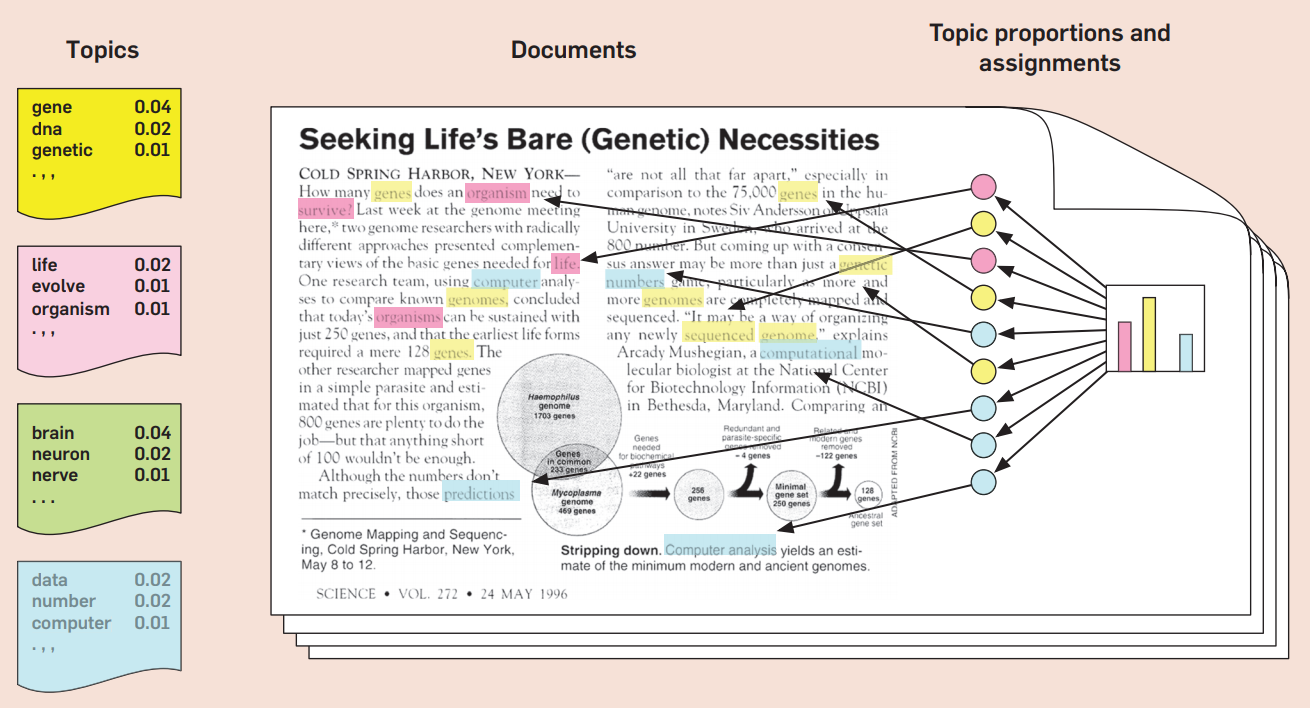
\includegraphics[width=0.8\textwidth]{document/images/lda_topic_model.png}
    % Der Teil in eckigen Klammern ist der Kurztitel für das Table of Contents
    \caption[Schematische Darstellung eines LDA Topic Modelings]{Schematische Darstellung eines LDA Topic Modelings. Quelle: \citetitle{blei_2012} \parencite{blei_2012}}
    \label{fig:lda_example}
\end{figure}

% Wenn wir nicht wollen, dass ein Kapitel auf einer neuen Seite startet, nutzen wir das hier:
{\let\clearpage\relax \chapter{Theoriefindung}}

\Blindtext

%% Bibliography

\setstretch{1.0}
\printbibliography[title={Literaturverzeichnis}]

\end{document}